\section{TITULO DA SECAO}\label{sec:diagnostico}
Além de citar referência bibliográfica com \cite{exemploArtigo}, você pode referenciar seções do relatório \autoref{sec:proposta} e \autoref{subsec:diagnostico}, figuras \autoref{fig:diagnostico-varias-imagens} e \autoref{fig:diagnostico-poli3}, tabelas \autoref{tab:diagnostico-exemplo} e equações \autoref{eq:diagnostico-relatividade}.

Exemplo de tabela:
\begin{table}[h!]
    \centering
    \caption{Tabela de exemplo}
    \begin{tabular}{cccc}
        \toprule
        \textbf{Item} & \textbf{Caracteristica 1} & \textbf{Caracteristica 2} & \textbf{Caracterista 3}\\
        \midrule
        x1 & y1 & z1 & w1\\
        x2 & y2 & z2 & w2\\
        \bottomrule
    \end{tabular}
    \label{tab:diagnostico-exemplo}
\end{table}

Exemplo de imagem:
\begin{figure}[h!]
    \centering
    \caption{Imagem de exemplo}
    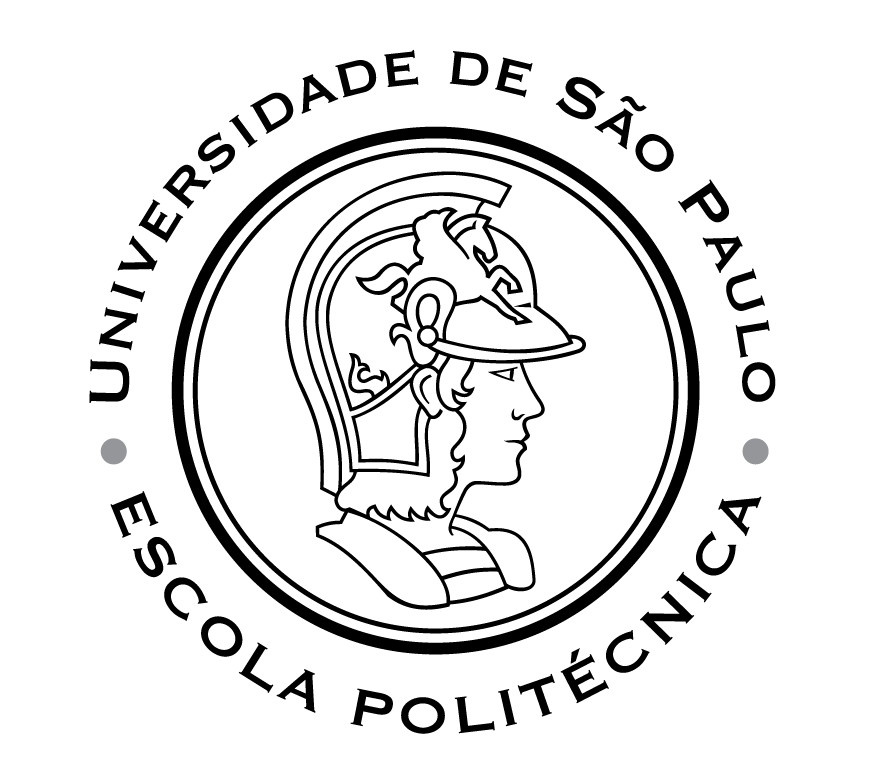
\includegraphics[width=0.5\textwidth]{imagens/Poli.png}
    \label{fig:diagnostico-poli}
    \source{\cite{exemploLivro}}
\end{figure}
Exemplo de equação:
\begin{equation}
    E = mc^2
    \label{eq:diagnostico-relatividade}
\end{equation}
Onde, \begin{itemize}
    \item $E$ é energia
    \item $m$ é massa
    \item $c=3\cdot10^3$ é a velocidade da luz no vácuo
\end{itemize}
\newpage Exemplo de multiplas imagens:
\begin{figure}[h!]
    \caption{Exemplo com varias imagens}
    \begin{subfigure}{0.5\textwidth}
        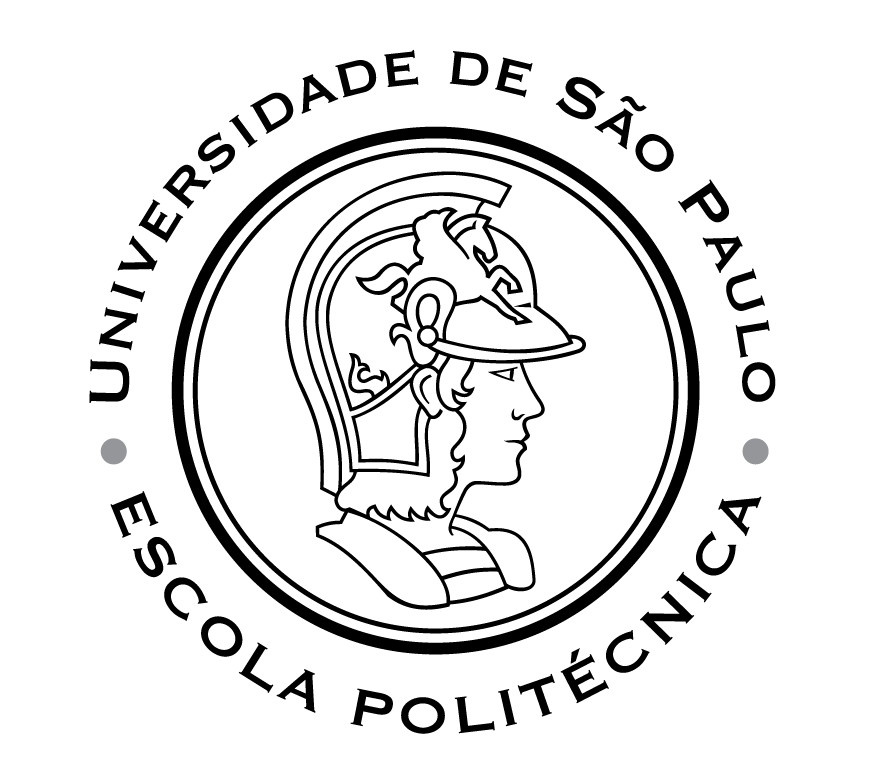
\includegraphics[width=0.9\textwidth]{imagens/Poli.png}
        \caption{Primeira imagem}
        \label{fig:diagnostico-poli1}
    \end{subfigure}%
    \begin{subfigure}{0.5\textwidth}
        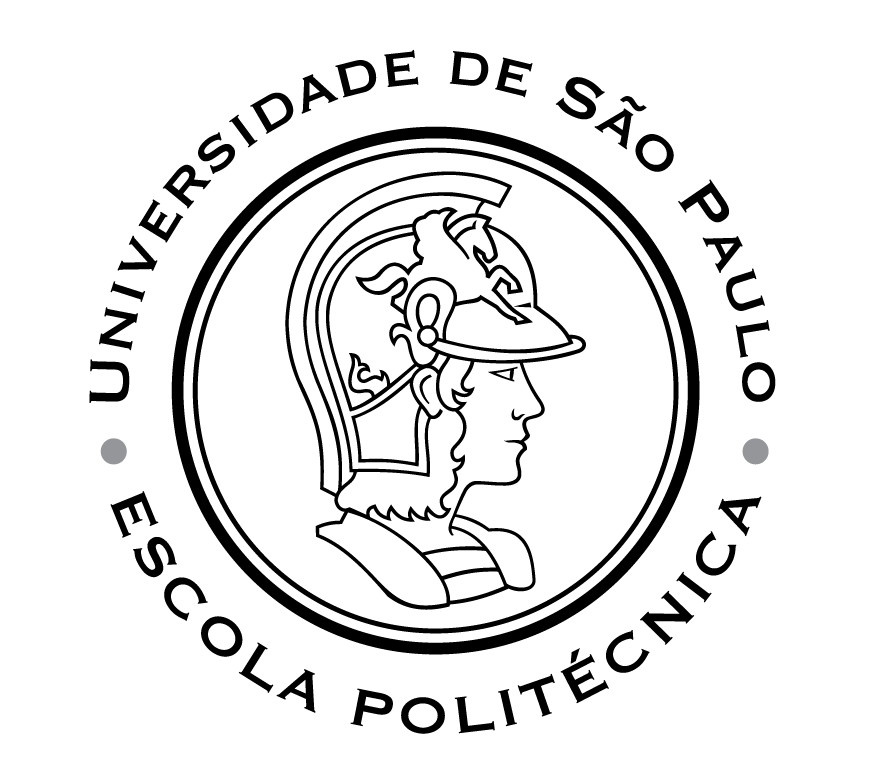
\includegraphics[width=0.9\textwidth]{imagens/Poli.png}
        \caption{Segunda imagem}
        \label{fig:diagnostico-poli2}
    \end{subfigure}
    \begin{subfigure}{0.5\textwidth}
        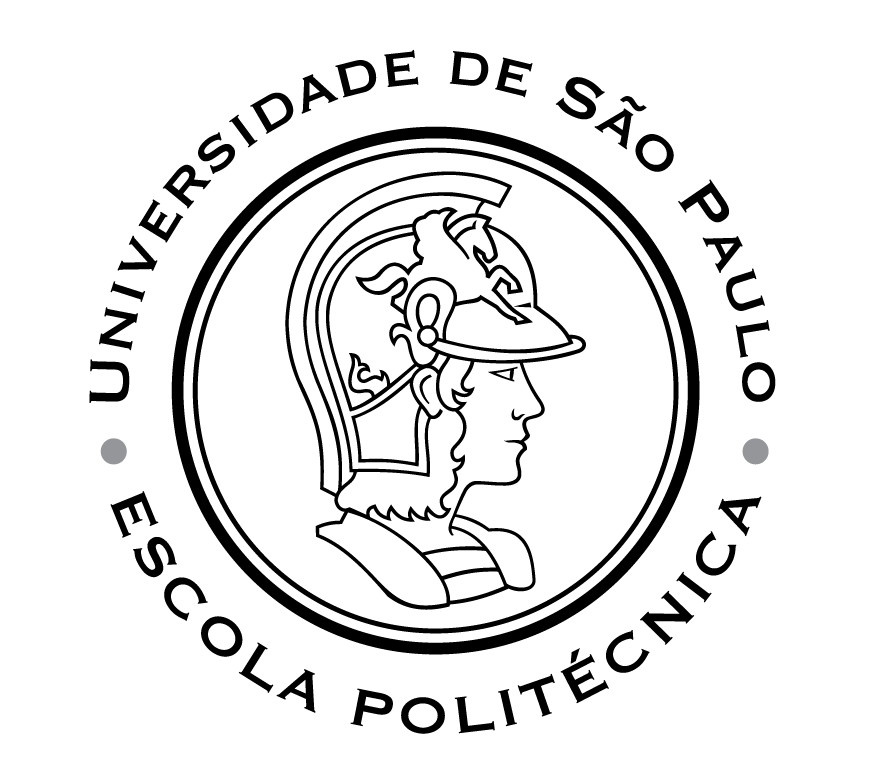
\includegraphics[width=0.9\textwidth]{imagens/Poli.png}
        \caption{Terceira imagem}
        \label{fig:diagnostico-poli3}
    \end{subfigure}
    \label{fig:diagnostico-varias-imagens}
    \source{Autor}
\end{figure}
\subsection{Titulo da Subsecao}\label{subsec:diagnostico}
\textit{[Texto de exemplo --- substituir pelo conteúdo real desta subseção.]}

\noindent\textbf{\textit{Titulo da subsubsecao 1}}

\textit{[Texto de exemplo --- substituir pelo conteúdo real desta subseção.]}
